% !TeX program = xelatex
% Draft status: DRAFT_NOT_SUBMISSION_READY
\documentclass[UTF8,a4paper,12pt]{ctexart}

\usepackage{geometry}
\geometry{top=2.4cm,bottom=2.4cm,left=2.5cm,right=2.5cm}
\usepackage{graphicx}
\usepackage{booktabs}
\usepackage{array}
\usepackage{amsmath,amssymb,bm}
\usepackage{siunitx}
\usepackage{caption}
\usepackage{enumitem}
\usepackage{setspace}
\usepackage{indentfirst}
\usepackage{titlesec}
\usepackage{natbib}
\usepackage{etoolbox}
\usepackage[hidelinks]{hyperref}
\usepackage{tikz}
\usetikzlibrary{arrows.meta,positioning,shapes.geometric}

\graphicspath{{figures/}}
\setlength{\parindent}{2em}
\setlength{\parskip}{0pt}
\linespread{1.25}
\captionsetup{font=small,labelsep=space,justification=centering,singlelinecheck=false}
\titleformat{\section}{\heiti\zihao{4}}{\thesection}{0.8em}{}
\titleformat{\subsection}{\heiti\zihao{-4}}{\thesubsection}{0.8em}{}
\titleformat{\subsubsection}{\heiti\zihao{-4}}{\thesubsubsection}{0.8em}{}
\setcitestyle{numbers,square,comma,super,sort&compress}
\AtBeginEnvironment{thebibliography}{\small\setlength{\itemsep}{0pt}\setlength{\parskip}{0pt}}

\newcommand{\zhabstract}[1]{\noindent\textbf{摘\quad 要：}#1\par}
\newcommand{\zhkeywords}[1]{\noindent\textbf{关键词：}#1\par}
\newcommand{\clc}[1]{\noindent\textbf{中图分类号：}#1\par}
\newcommand{\enabstract}[1]{\noindent\textbf{Abstract: }#1\par}
\newcommand{\enkeywords}[1]{\noindent\textbf{Keywords: }#1\par}
\newcommand{\bicaption}[2]{\caption{#1\\[-0.2em]\small Fig.\thefigure\ #2}}
\newcommand{\bitablecaption}[2]{\caption{#1\\[-0.2em]\small Table \thetable\ #2}}
\newcommand{\simdefault}{\texttt{simulation/default}}

\begin{document}

\begin{center}
{\heiti\zihao{2}\textbf{光栅扭矩测量全链路数字孪生与算法评估}\par}
\vspace{0.8em}
{\zihao{4} 作者信息待补$^{1,2}$\par}
\vspace{0.5em}
{\zihao{-5}（1. 单位信息待补，省市邮编待补；2. 合作单位信息待补，省市邮编待补）\par}
\end{center}

\vspace{0.8em}

\zhabstract{针对光栅扭矩测量中机械参数、光电非理想误差和环境温度变化相互耦合，导致算法比较难以复现、温漂补偿难以在同一测量链中验证的问题，本文建立了一套面向光栅扭矩测量的全链路数字孪生仿真平台。平台按照“扭矩输入—扭转角—光栅相对位移—光学相位—四相信号—误差注入—ADC量化—协议帧”的顺序组织机械、光学、信号和通信模型，并以五通道零位/分相信号作为计数细分算法的仿真基线。在统一随机种子和参数快照下，构建理想、幅值失配、相位误差、直流偏置、信噪比为30、20和10 dB以及正反向扭矩扫描等14类工况，对1/4、1/16、1/32分相计数、差分反正切和协方差白化改进法进行对比。结果表明，在当前仿真默认参数下，1/32分相计数基线的全工况平均位移RMSE为$0.384~\si{\micro\metre}$，最大RMSE为$0.728~\si{\micro\metre}$，对应工况为SNR=10 dB；差分反正切和改进法的最大RMSE分别出现在$-1~\si{\newton\metre}$反向扭矩扫描中。进一步在$-20$~$80~^\circ\mathrm{C}$范围内引入剪切模量和光栅周期的一阶温度模型，得到未补偿灵敏度变化范围为$-1.186\%$至$+1.833\%$，最大扭矩RMSE为$0.084655~\si{\newton\metre}$；使用同一模型参数进行逆补偿后，计算误差回到数值零附近。上述结果只说明当前模型和默认系数下的仿真规律，不能替代实物标定、真实温箱实验或COM端口通信验证。}

\vspace{0.4em}
\zhkeywords{光栅扭矩测量；数字孪生；四相信号；分相计数；温度补偿；仿真验证}
\clc{TP212；TH741}

\vspace{1em}
\begin{center}
{\bfseries\large Full-Pipeline Digital Twin and Algorithm Evaluation for Optical Grating Torque Measurement\par}
\vspace{0.6em}
Author information to be completed$^{1,2}$\par
\vspace{0.4em}
\small
(1. Affiliation to be completed; 2. Affiliation to be completed)\par
\end{center}

\enabstract{A full-pipeline digital-twin simulation platform was developed for optical grating torque measurement, where mechanical parameters, optoelectronic nonidealities, and temperature variations are coupled in the measurement chain. The platform follows the sequence of torque input, torsional deformation, grating displacement, optical phase, four-phase sensing, error injection, ADC quantization, and protocol framing. A five-channel zero-reference and phase-subdivision model was used as the simulation baseline. Under fixed parameter snapshots and random seeds, 14 operating cases were constructed, including nominal signals, amplitude mismatch, phase error, DC offset, SNR levels of 30, 20, and 10 dB, and positive/negative torque sweeps. Five methods were compared: 1/4, 1/16, and 1/32 phase-subdivision counting, differential atan2, and a covariance-whitening method with median offset removal and RMS normalization. Under the current simulation/default parameters, the 1/32 counting baseline achieved a mean displacement RMSE of $0.384~\si{\micro\metre}$ and a worst-case RMSE of $0.728~\si{\micro\metre}$, with the worst case at SNR=10 dB. The largest RMSEs of the two continuous phase methods occurred in the $-1~\si{\newton\metre}$ reverse-torque sweep. A first-order temperature model was then introduced over $-20$ to $80~^\circ\mathrm{C}$. The uncompensated sensitivity variation ranged from $-1.186\%$ to $+1.833\%$, and the maximum torque RMSE was $0.084655~\si{\newton\metre}$. Model-based inverse compensation reduced the calculated error to the numerical-zero level. These results describe the behavior of the present simulation model and unverified default coefficients; they do not constitute physical calibration, chamber testing, or real COM communication evidence.}

\vspace{0.4em}
\noindent\textbf{Keywords: }optical grating torque measurement; digital twin; quadrature signal; phase subdivision; temperature compensation; simulation validation

\section*{引言}

扭矩是旋转机械动力传递、状态监测和闭环控制中的重要测量量。基于光栅或莫尔条纹的非接触测量具有抗电磁干扰和高分辨率等特点，但其输出精度并不只由光栅周期决定，还受到扭轴刚度、安装半径、通道增益、直流偏置、正交相位和噪声等因素共同影响。对于这类力学变形、光学调制和电信号处理连续耦合的系统，单独考察某一算法或某一理想信号，难以解释测量链在参数失配、反向运动和温度变化条件下的整体行为。

数字孪生技术为传感器的机理建模、虚拟调试和极端工况测试提供了统一载体。已有研究围绕数字孪生的体系结构和工程应用开展了较系统的讨论\cite{ref1,ref2}；光电位移和轴角测量研究则重点关注正交信号误差、细分误差及椭圆轨迹校正\cite{ref3,ref4,ref5,ref6,ref7,ref9,ref10,ref11}。然而，已有工作通常分别讨论机械模型、解调算法或误差补偿，缺少将“载荷—位移—相位—光电信号—ADC—协议帧”连成一个可重复执行的测量链，并对仿真参数、数据文件和异常记录进行统一管理的研究框架。

本文关注一个参数化光栅扭矩测量系统，研究重点不是声称完成特定实物的尺寸复原，而是建立带参数来源标记的仿真基准，回答三个问题：第一，如何把扭矩、光栅相位和数字采样统一到可追溯的计算链中；第二，在相同输入和随机种子下，不同解调方法在非理想工况中的误差差异如何；第三，若将材料剪切模量和光栅周期的温度变化显式纳入模型，前馈逆补偿能在多大程度上抑制模型内的温漂误差。

本文主要工作如下：
\begin{enumerate}[label=（\arabic*）,leftmargin=3em]
  \item 建立从扭矩到四相信号、ADC和11字节旧版协议帧的全链路数字孪生模型，并明确机械尺寸、材料参数和温度系数均为当前 \simdefault 仿真假设；
  \item 基于当前 MATLAB 数据文件构建14类工况、5种解调方法和70条记录的可复现比较，保留零扭矩静态点的秩亏警告，不按结果删除异常行；
  \item 建立一阶温度漂移模型，比较补偿前后的模型内误差，并明确软件闭环、协议帧预览和真实硬件通信之间的证据边界。
\end{enumerate}

\section{全链路数字孪生模型}

\subsection{平台架构与参数来源}

平台由 MATLAB 计算层和 Python/VTK 交互层组成。MATLAB 层负责机械映射、光学相位、四相信号、非理想误差、ADC量化、解调算法和数据报告；Python 层负责参数输入、参数化装配显示、MATLAB Engine 调用和协议帧预览。完整信息流如图\ref{fig:architecture}所示。

\begin{figure}[htbp]
  \centering
  \begin{tikzpicture}[node distance=0.7cm and 0.32cm, >=Stealth,
    block/.style={rectangle,draw=black,minimum width=2.25cm,minimum height=0.85cm,align=center,font=\small},
    line/.style={draw=black,-{Stealth[length=2mm]}}]
    \node[block] (t) {扭矩输入\\$T$};
    \node[block,right=of t] (m) {扭转力学\\$\theta,x_{\rm rel}$};
    \node[block,right=of m] (o) {光学相位\\$\phi$};
    \node[block,right=of o] (s) {四相信号\\误差注入};
    \node[block,right=of s] (a) {ADC\\量化};
    \node[block,right=of a] (c) {协议帧\\预览};
    \node[block,below=of o] (temp) {温度输入\\$T_{\rm e}$};
    \node[block,below=of s] (alg) {解调\\RMSE/鲁棒性};
    \path[line](t)--(m); \path[line](m)--(o); \path[line](o)--(s); \path[line](s)--(a); \path[line](a)--(c);
    \path[line](temp)--(m); \path[line](temp)--(alg); \path[line](s)--(alg);
  \end{tikzpicture}
  \bicaption{光栅扭矩测量全链路数字孪生架构}{Full-pipeline digital-twin architecture for optical grating torque measurement}
  \label{fig:architecture}
\end{figure}

专利资料只用于约束部件功能关系和通道语义，当前模型中的扭轴、腔体、光栅盘和传感器位姿不能解释为专利实物尺寸复原。所有未由图纸、材料证书或实物标定确认的数值均标记为 \simdefault。用于阶段14和阶段15的主要参数见表\ref{tab:parameters}。

\begin{table}[htbp]
  \centering
  \bitablecaption{当前仿真使用的主要参数及来源}{Main simulation parameters and their sources}
  \label{tab:parameters}
  \begin{tabular}{lccc}
    \toprule
    参数 & 符号 & 数值 & 来源/单位 \\
    \midrule
    有效扭转段长度 & $L$ & $0.012$ & \simdefault / m \\
    扭轴直径 & $d$ & $0.008$ & \simdefault / m \\
    剪切模量 & $G_0$ & $79$ & \simdefault / GPa \\
    有效检测半径 & $r_{\rm eff}$ & $0.007$ & \simdefault / m \\
    光栅周期 & $P_0$ & $20$ & \simdefault / $\si{\micro\metre}$ \\
    单次采样点数 & $M$ & $2001$ & 仿真设置 / 点 \\
    单次仿真时长 & $t_{\rm end}$ & $1$ & 仿真设置 / s \\
    ADC分辨率与量程 & $N,[V_{\min},V_{\max}]$ & $12,[0,3.3]$ & 仿真设置 / bit,V \\
    随机种子起点 & $s_0$ & $20260916$ & 数据记录 / -- \\
    \bottomrule
  \end{tabular}
\end{table}

\subsection{扭矩、位移与光学相位映射}

将扭轴视为圆截面弹性轴，极惯性矩为
\begin{equation}
  J=\frac{\pi d^4}{32}.
  \label{eq:polar}
\end{equation}
在小变形和线性弹性假设下，输入扭矩与扭转角的关系为
\begin{equation}
  \theta=\frac{TL}{GJ}.
  \label{eq:torsion}
\end{equation}
有效检测半径处的切向相对位移为
\begin{equation}
  x_{\rm rel}=x_{\rm bias}+r_{\rm eff}\theta,
  \label{eq:displacement}
\end{equation}
光栅相对位移进一步转换为光学相位
\begin{equation}
  \phi=\frac{2\pi x_{\rm rel}}{P}+\phi_0.
  \label{eq:phase}
\end{equation}
式中，$T$为输入扭矩，$L$为有效扭转段长度，$G$为剪切模量，$d$为扭轴直径，$r_{\rm eff}$为有效检测半径，$P$为光栅周期，$x_{\rm bias}$和$\phi_0$分别为位移和相位初始偏置。上述关系是当前平台的集中参数模型，尚未包含热梯度、装配应力和轴向耦合。

\subsection{四相光电信号与非理想误差}

四个测量通道的理想相位偏置为$0$、$\pi/2$、$\pi$和$3\pi/2$，理想信号可写为
\begin{equation}
  u_i(t)=I_0+I_m\cos\left(\phi(t)+\varphi_i\right),\quad
  \varphi_i\in\left\{0,\frac{\pi}{2},\pi,\frac{3\pi}{2}\right\}.
  \label{eq:fourphase}
\end{equation}
平台的误差层按通道注入幅值系数、相位偏差、直流偏置和高斯噪声；同时保留高频干扰接口。阶段14基准实验实际使用了幅值失配、相位误差、直流偏置和高斯噪声，未将高次谐波作为该批14类统计中的独立工况。统一写成
\begin{equation}
  u_i^*(t)=A_i\cos\left(\phi(t)+\varphi_i+\delta_i\right)+B_i+n_i(t)+h(t),
  \label{eq:error}
\end{equation}
其中，$A_i$、$\delta_i$和$B_i$分别为通道幅值、相位误差和直流偏置，$n_i(t)$为高斯噪声，$h(t)$为可选的公共干扰项。信号经过限幅和均匀量化后得到
\begin{equation}
  D_i=\operatorname{round}\left[\frac{\operatorname{clip}(u_i^*,V_{\min},V_{\max})-V_{\min}}{V_{\max}-V_{\min}}(2^N-1)\right].
  \label{eq:adc}
\end{equation}

\subsection{协议帧与软件闭环边界}

现有旧版协议帧为
\begin{center}
\texttt{AA | A\_H A\_L | B\_H B\_L | C\_H C\_L | D\_H D\_L | CRC\_H CRC\_L}.
\end{center}
每帧11字节，数据为四路大端16位ADC码，校验为CRC-16/CCITT-FALSE。阶段16验收报告记录了GUI/VTK装配、MATLAB Engine、信号、ADC和帧生成/预览的联动，测试波形为41点，ADC矩阵为$41\times4$。该结果证明软件闭环和协议编码可运行，但由于未打开真实COM端口，不能写成硬件串口通信实测；同样，协议帧预览不能替代STM32接收或物理传感器输出验证。

\section{解调方法与评价指标}

\subsection{五通道分相计数基线}

为模拟带零位参考的分相检测结构，平台生成\texttt{ZERO}、\texttt{MAIN}、\texttt{PHASE\_90}、\texttt{PHASE\_180}和\texttt{PHASE\_270}五个通道。四个相位通道通过差分组合形成相位轨迹，零位通道用于确定参考位置。平台分别输出1/4、1/16和1/32计数结果，其名义位移步长为$P/4$、$P/16$和$P/32$；当$P=20~\si{\micro\metre}$时，1/32步长为$0.625~\si{\micro\metre}$。这里的五通道模型是仿真基线，不表示现有ADC和串口接口已经扩展为五通道。

\subsection{差分反正切基线}

将四相信号作互补差分，得到
\begin{equation}
  u=\frac{u_A-u_C}{2},\qquad v=\frac{u_D-u_B}{2}.
  \label{eq:diff}
\end{equation}
再利用反正切和相位展开求取位移：
\begin{equation}
  \hat{x}_{\rm atan2}=\frac{P}{2\pi}\operatorname{unwrap}\left[\operatorname{atan2}(v-\bar v,u-\bar u)\right].
  \label{eq:atan2}
\end{equation}
该方法结构简单，但对幅值失配、直流偏置、正交误差和相位展开边界较敏感。

\subsection{协方差白化改进法}

当前实现首先对每个通道进行中值去偏和RMS归一化，再在二维差分轨迹上计算协方差矩阵，并利用特征分解构造白化矩阵，使轨迹在仿真中接近单位圆，最后使用反正切和相位展开恢复位移。该方法在本文中称为“协方差白化改进法”，不将其直接等同于完整的代数椭圆拟合算法，以保持方法名称与代码实现一致。

\subsection{评价指标}

设真实位移为$x_m$，估计位移为$\hat{x}_m$，样本数为$M$，则RMSE、MAE和最大误差分别为
\begin{equation}
  \mathrm{RMSE}=\sqrt{\frac{1}{M}\sum_{m=1}^{M}(\hat{x}_m-x_m)^2},
  \label{eq:rmse}
\end{equation}
\begin{equation}
  \mathrm{MAE}=\frac{1}{M}\sum_{m=1}^{M}|\hat{x}_m-x_m|,\qquad
  e_{\max}=\max_m|\hat{x}_m-x_m|.
  \label{eq:mae}
\end{equation}
为便于比较不同工况，沿用数据报告中的归一化鲁棒性评分
\begin{equation}
  S_{\rm rob}=\frac{1}{1+\mathrm{RMSE}/(P/32)}.
  \label{eq:robustness}
\end{equation}
当算法触发可辨识性警告时，鲁棒性评分不参与均值计算，但对应记录仍保留在原始结果文件中。

\section{仿真设计与可复现性}

\subsection{14类工况矩阵}

阶段14使用2001个采样点、1 s仿真时长和以20260916为起点的逐工况随机种子。14类工况由理想、参数失配、噪声和扭矩扫描四组组成，具体见表\ref{tab:cases}。

\begin{table}[htbp]
  \centering
  \bitablecaption{阶段14实际执行的14类仿真工况}{Fourteen simulation cases actually executed in Stage 14}
  \label{tab:cases}
  \begin{tabular}{clp{7.2cm}}
    \toprule
    编号 & 标识 & 参数或输入 \\
    \midrule
    C01 & ideal & 四通道幅值0.8，无偏置、无相位误差、无噪声，$T_{\rm peak}=8$ N.m \\
    C02 & amplitude\_mismatch & 四通道幅值为$[0.52,1.08,0.64,0.96]$ \\
    C03 & phase\_error & 相位误差为$[0.15,-0.12,0.08,-0.10]$ rad \\
    C04 & dc\_offset & 直流偏置为$[0.15,-0.10,0.08,-0.05]$ \\
    C05--C07 & snr\_30/20/10dB & 高斯噪声，SNR分别为30、20和10 dB \\
    C08--C14 & torque sweep & 峰值扭矩依次为$-8,-4,-1,0,1,4,8$ N.m \\
    \bottomrule
  \end{tabular}
\end{table}

所有方法在同一工况中使用相同的真实位移轨迹、信号扰动和随机种子。结果文件保留14个工况与5种方法的全部70条记录；当前数据中有69条为\texttt{ok}，有1条为\texttt{warning}，没有因结果不佳而删除记录。

\subsection{温度模型与补偿对照}

温度仿真在$-20$、0、20、40、60和80 $^\circ$C进行。以20 $^\circ$C为参考，剪切模量和光栅周期采用一阶模型
\begin{equation}
  G(T_{\rm e})=G_0[1+\alpha_G(T_{\rm e}-T_0)],
  \qquad
  P(T_{\rm e})=P_0[1+\alpha_P(T_{\rm e}-T_0)].
  \label{eq:temperature}
\end{equation}
其中$\alpha_G=-3.0\times10^{-4}~^\circ\mathrm{C}^{-1}$，$\alpha_P=1.2\times10^{-5}~^\circ\mathrm{C}^{-1}$。两项系数均为未验证的仿真默认参数。补偿关闭时使用$G_0$和$P_0$，补偿开启时使用温度更新后的$G(T_{\rm e})$和$P(T_{\rm e})$进行逆变换。该设计适合验证模型内部一致性，不足以证明实际材料的温度响应服从式\eqref{eq:temperature}。

\section{结果与讨论}

\subsection{解调算法总体比较}

表\ref{tab:method}汇总了阶段14报告中的统计结果。1/32分相计数的平均RMSE和最差RMSE均低于另外两种分相计数基线；两种连续相位方法的中位数RMSE较低，但在反向扭矩扫描中出现较大的最差误差。表中改进法的均值沿用原始报告口径，其中零扭矩行虽然输出RMSE为0，但状态为秩亏警告，因此该均值不能解释为所有工况均无可辨识性问题。

\begin{table}[htbp]
  \centering
  \bitablecaption{五种方法在14类工况下的统计结果}{Statistics of five methods over the 14 operating cases}
  \label{tab:method}
  \resizebox{\textwidth}{!}{%
  \begin{tabular}{lcccccc}
    \toprule
    方法 & 保留记录 & 平均RMSE/$\si{\micro\metre}$ & 中位数RMSE/$\si{\micro\metre}$ & 最大RMSE/$\si{\micro\metre}$ & 鲁棒性均值 & 最差工况 \\
    \midrule
    1/4分相计数 & 14/14 ok & 2.419 & 2.808 & 3.009 & 0.256 & snr\_10dB \\
    1/16分相计数 & 14/14 ok & 0.686 & 0.712 & 1.007 & 0.500 & snr\_10dB \\
    1/32分相计数 & 14/14 ok & 0.384 & 0.360 & 0.728 & 0.638 & snr\_10dB \\
    差分反正切 & 14/14 ok & 1.334 & 0.365 & 5.698 & 0.578 & torque\_neg1Nm \\
    协方差白化改进法 & 13 ok+1 warning & 1.730 & 0.148 & 7.748 & 0.565 & torque\_neg1Nm \\
    \bottomrule
  \end{tabular}%
  }
\end{table}

图\ref{fig:rmse}给出了各工况的RMSE分布。对于当前模型，1/32分相计数在噪声增强时的误差增长较为平缓，SNR=10 dB时仍保持$0.728~\si{\micro\metre}$的最大RMSE。该结果只能说明离散计数基线在本组输入和参数下具有较好的抗扰表现，不能外推为真实传感器的分辨率或精度指标。

\begin{figure}[htbp]
  \centering
  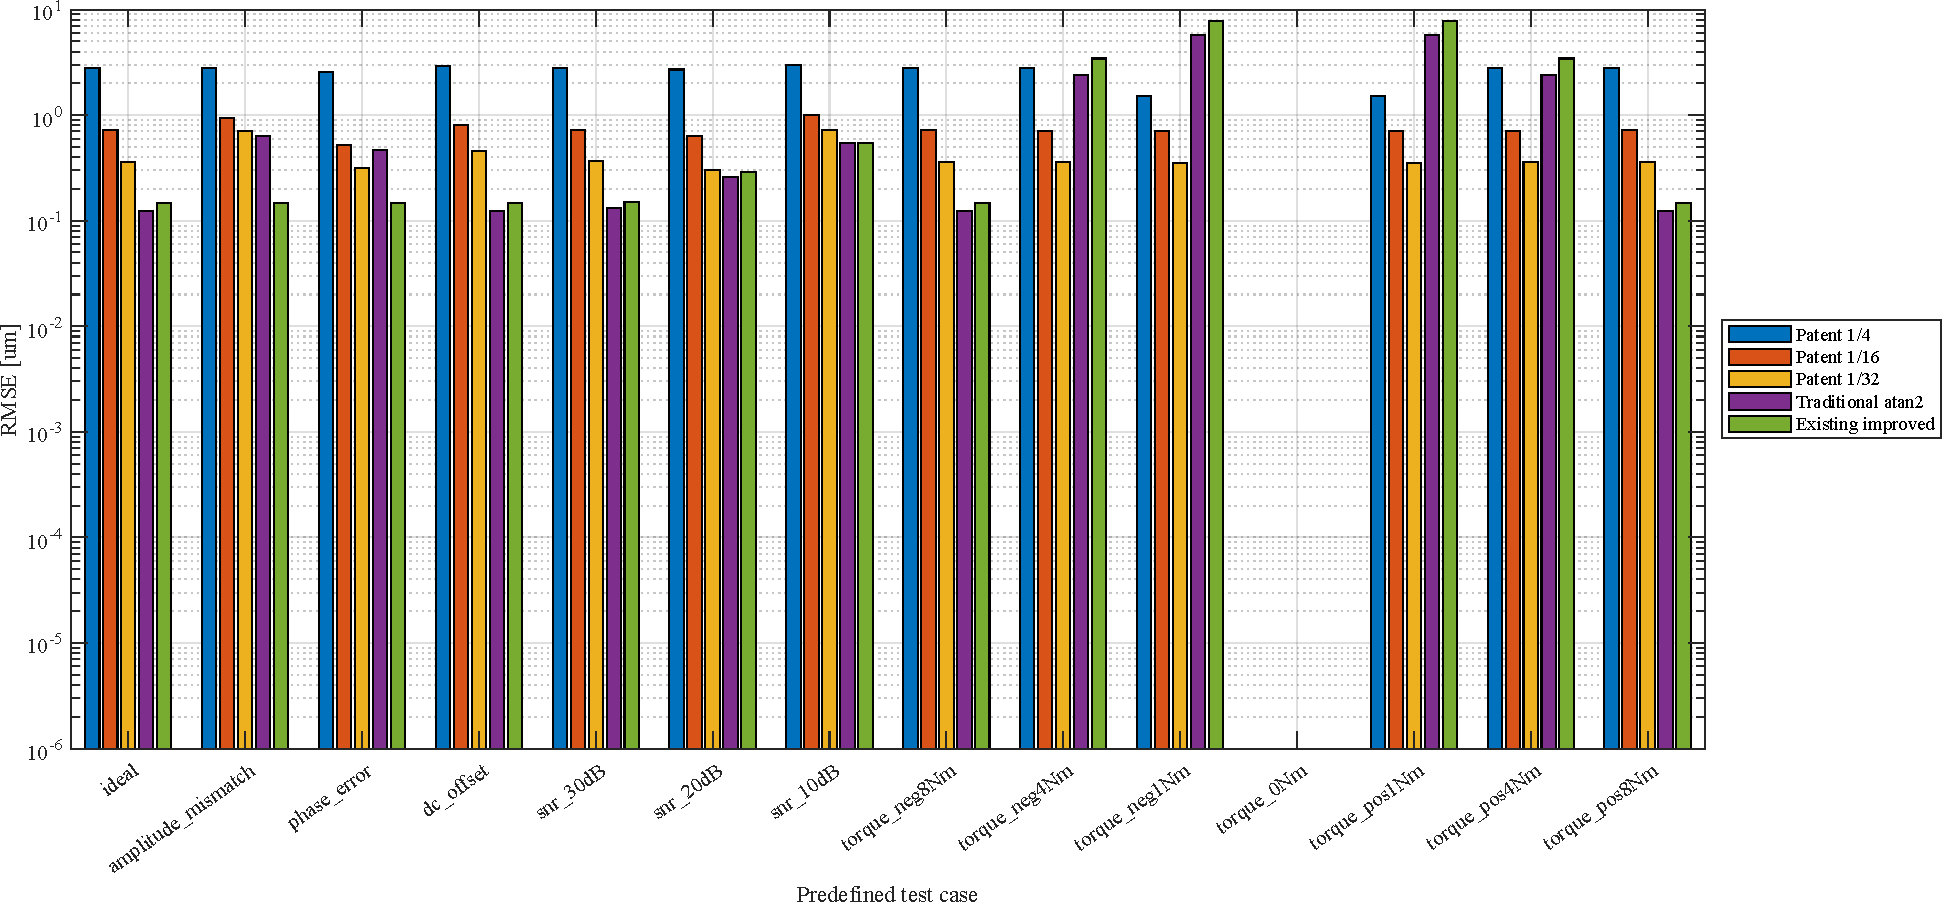
\includegraphics[width=0.88\linewidth]{stage14_rmse_all_cases.pdf}
  \bicaption{14类工况下五种解调方法的位移RMSE}{Displacement RMSE of five demodulation methods over 14 cases}
  \label{fig:rmse}
\end{figure}

\subsection{误差曲线、反向扭矩与静态奇异点}

图\ref{fig:errors}展示了典型工况下的误差曲线。分相计数方法的误差呈现由步长约束形成的离散轨迹，而连续相位方法的误差受相位展开和轨迹形状影响更明显。阶段14数据中，差分反正切和协方差白化改进法的最大RMSE分别发生在$-1$ N.m反向扭矩扫描，提示在当前实现中，方向变化与相位展开边界需要单独进行动态验证。

\begin{figure}[htbp]
  \centering
  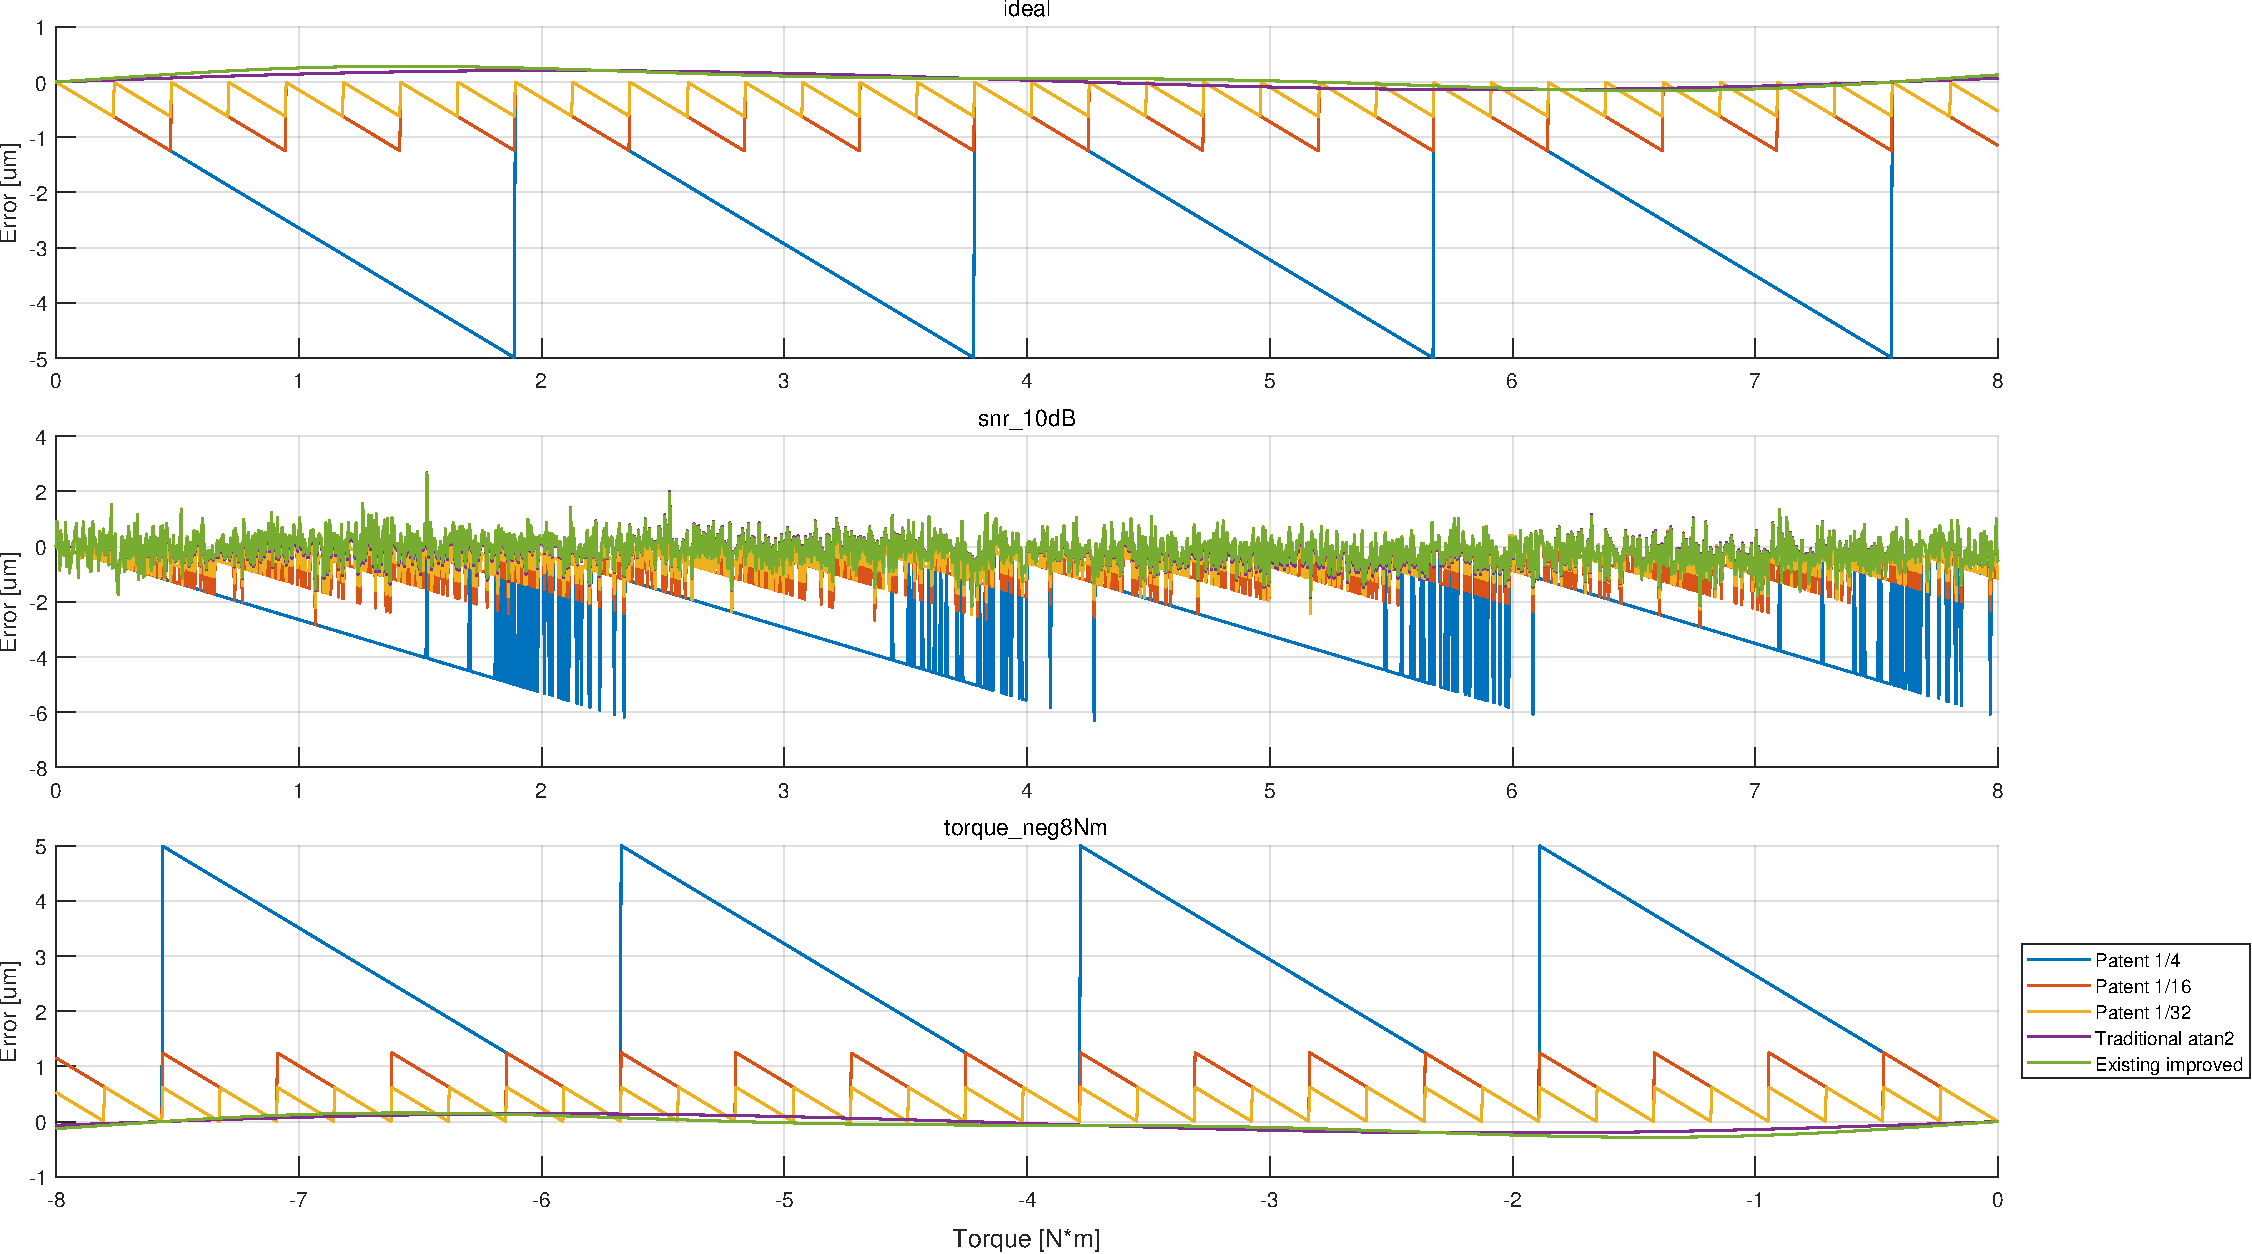
\includegraphics[width=0.88\linewidth]{stage14_error_curves.pdf}
  \bicaption{典型工况下的位移估计误差曲线}{Displacement estimation errors under representative cases}
  \label{fig:errors}
\end{figure}

在$T=0$的静态工况中，协方差白化改进法产生了\texttt{rankDeficientMatrix}警告，报告记录秩为1。根据当前模型，零扭矩时相位轨迹不随时间展开，二维信号点集退化，依赖协方差和矩阵求解的校正步骤缺少足够的几何信息，这是该警告的合理模型内解释。该解释仍需在真实静态噪声和有限采样条件下进一步验证；在工程实现中，宜为静态点设置保持逻辑或切换到不依赖轨迹拟合的解调路径。

\begin{figure}[htbp]
  \centering
  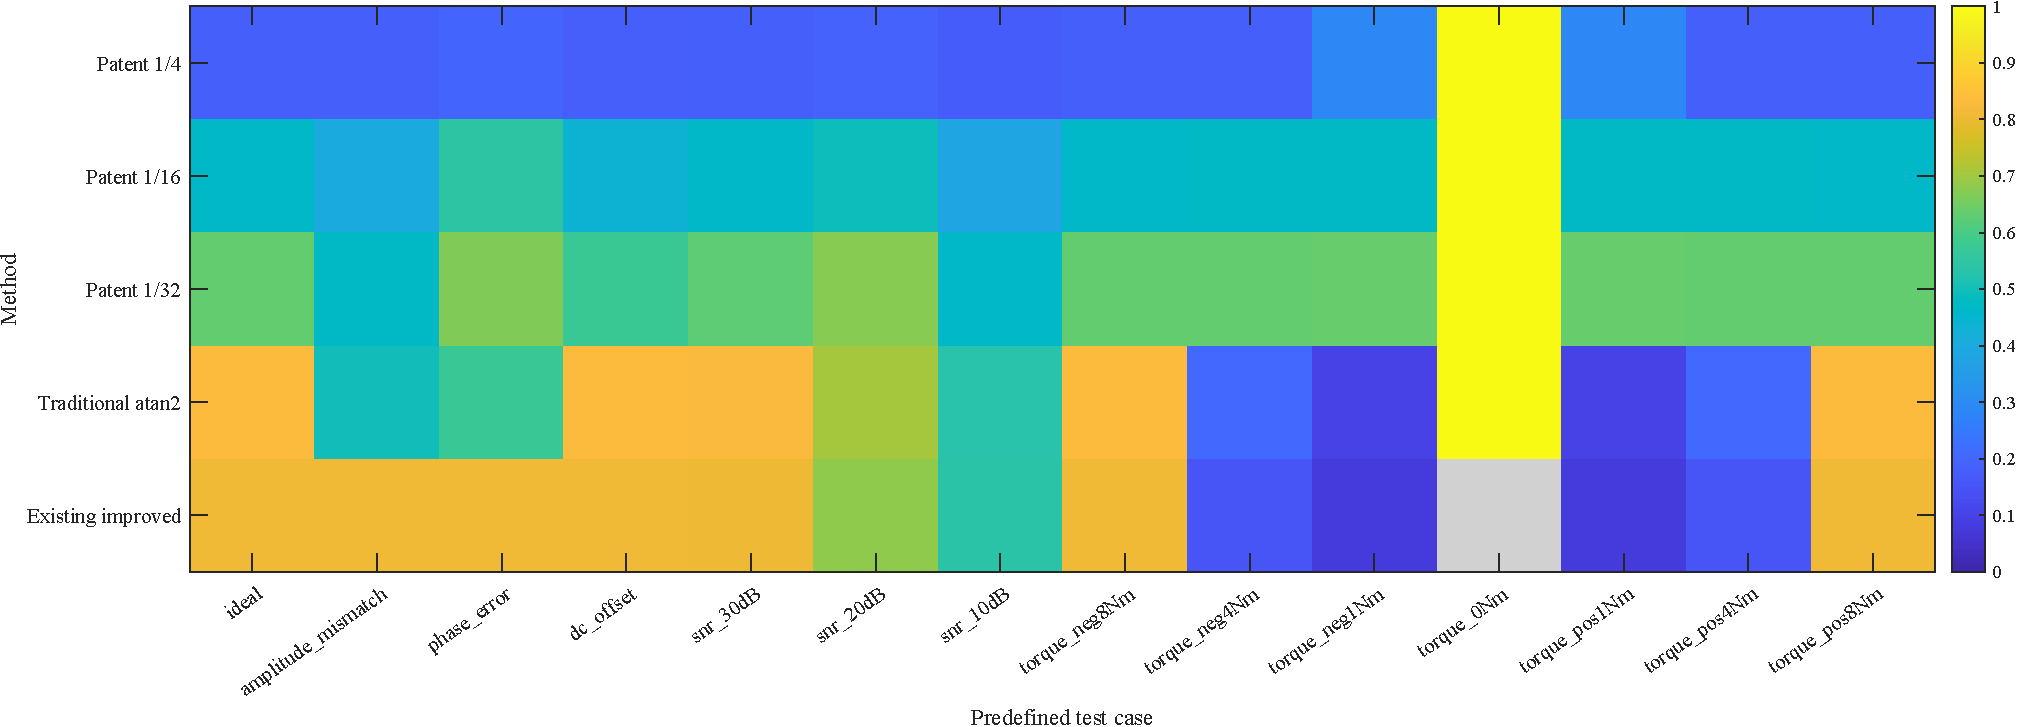
\includegraphics[width=0.84\linewidth]{stage14_robustness_score.pdf}
  \bicaption{不同工况下的归一化鲁棒性评分}{Normalized robustness scores under different cases}
  \label{fig:robustness}
\end{figure}

\subsection{温度漂移与模型内补偿效果}

图\ref{fig:temperature}给出了剪切模量和灵敏度变化。温度从20 $^\circ$C下降到$-20~^\circ$C时，模型灵敏度相对变化为$-1.1858\%$；升高到80 $^\circ$C时为$+1.8330\%$。图\ref{fig:compensation}和表\ref{tab:temperature}给出了补偿前后的扭矩误差。未补偿最大扭矩RMSE为$0.084655~\si{\newton\metre}$，出现在80 $^\circ$C；最大瞬时误差为$0.140778~\si{\newton\metre}$。补偿开启后，CSV中的扭矩RMSE为0或数值零附近。

\begin{figure}[htbp]
  \centering
  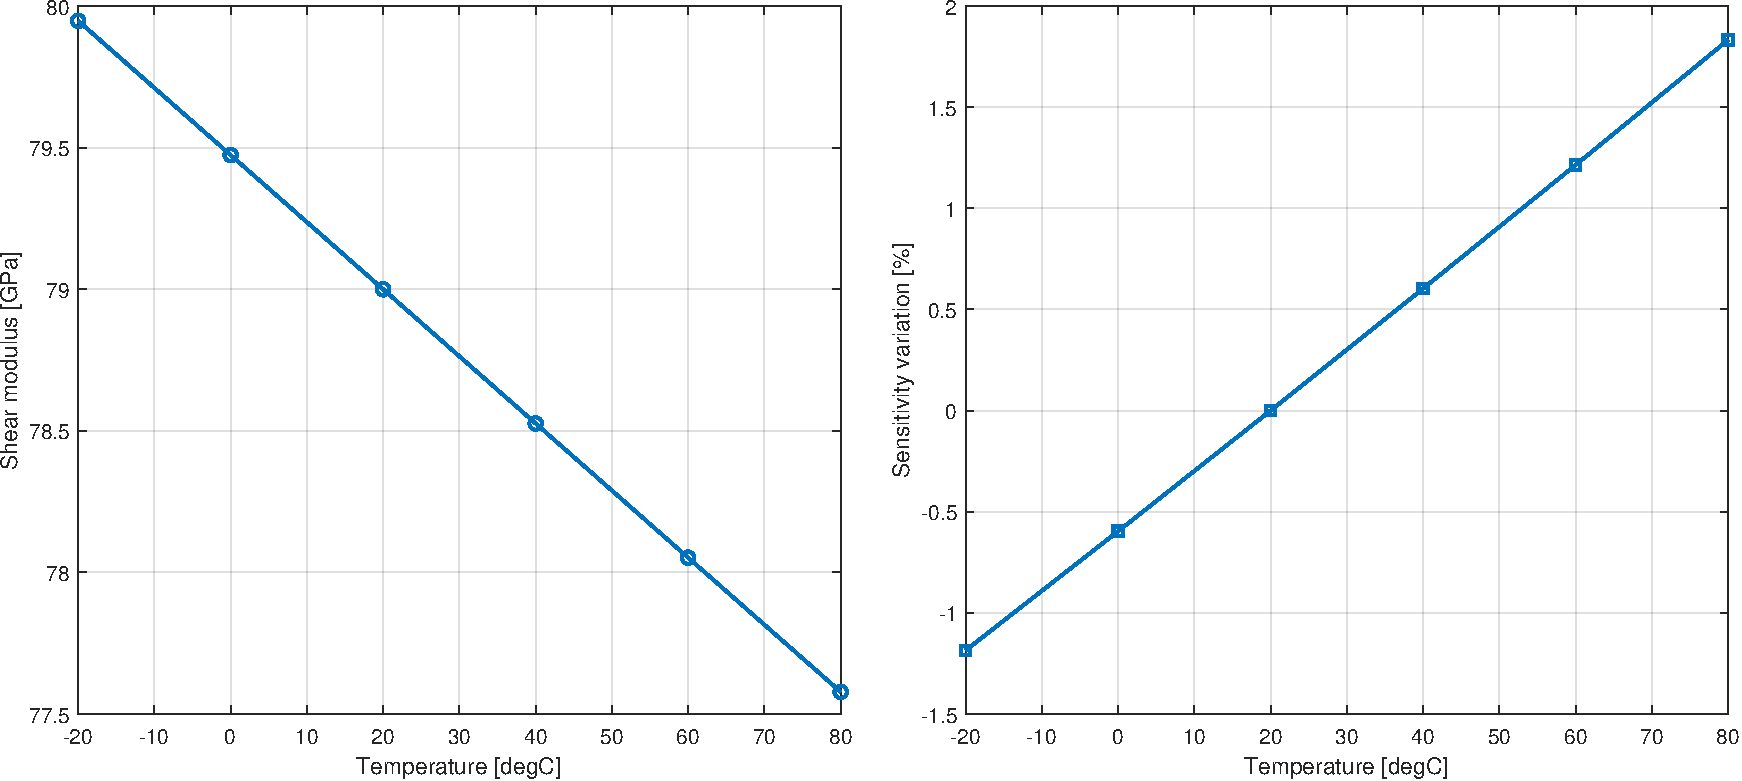
\includegraphics[width=0.82\linewidth]{stage15_material_sensitivity.pdf}
  \bicaption{温度对剪切模量和测量灵敏度的仿真影响}{Simulated temperature effects on shear modulus and measurement sensitivity}
  \label{fig:temperature}
\end{figure}

\begin{figure}[htbp]
  \centering
  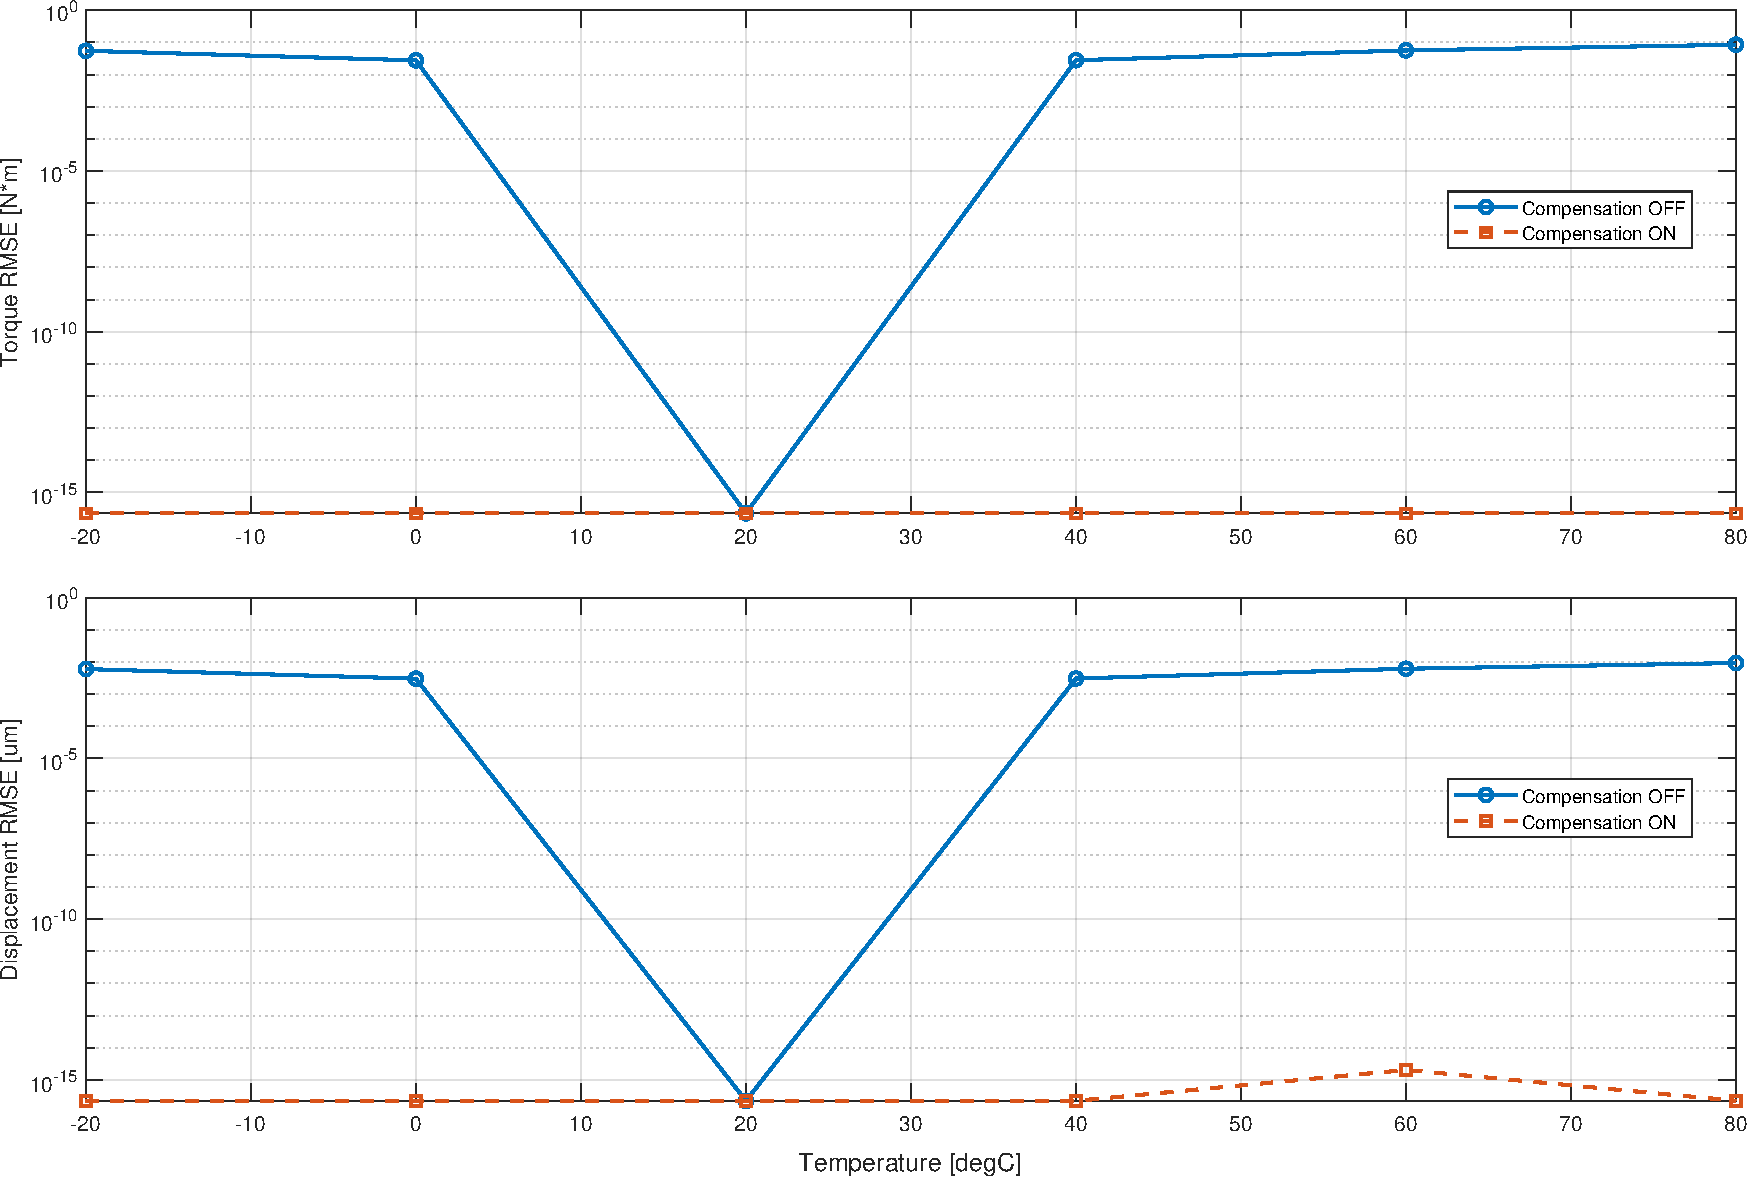
\includegraphics[width=0.82\linewidth]{stage15_compensation_rmse.pdf}
  \bicaption{温度补偿前后的扭矩RMSE}{Torque RMSE before and after temperature compensation}
  \label{fig:compensation}
\end{figure}

\begin{table}[htbp]
  \centering
  \bitablecaption{不同温度下的灵敏度变化和扭矩误差}{Sensitivity variation and torque errors at different temperatures}
  \label{tab:temperature}
  \begin{tabular}{ccccc}
    \toprule
    温度/$^\circ$C & $G$/GPa & 灵敏度变化/\% & 未补偿RMSE/N.m & 补偿后RMSE/N.m \\
    \midrule
    -20 & 79.948 & -1.186 & 0.054761 & 0 \\
    0 & 79.474 & -0.596 & 0.027544 & 0 \\
    20 & 79.000 & 0.000 & 0 & 0 \\
    40 & 78.526 & 0.604 & 0.027877 & 0 \\
    60 & 78.052 & 1.215 & 0.056094 & 0 \\
    80 & 77.578 & 1.833 & 0.084655 & 0 \\
    \bottomrule
  \end{tabular}
\end{table}

需要强调的是，补偿前后使用的是同一套温度模型和同一组未验证系数，补偿结果反映的是模型内部参数逆变换的一致性，而不是实际材料和光栅在温箱中的测量结果。要将该结果提升为工程性能结论，至少还需要温度循环实验、材料参数辨识、光栅周期实测和多次重复数据。

\subsection{结果的工程含义与证据边界}

本文结果具有两层含义。第一层是方法学含义：将机械、光学、信号和协议模块置于同一参数快照下，可以把算法比较从孤立信号测试推进到可追溯的测量链测试，并能保留异常工况。第二层是当前模型的定量观察：1/32分相计数在14类仿真工况中得到较低的平均和最差RMSE，温度逆补偿可以消除由指定系数引入的模型内偏差。

但下列结论尚不能由当前证据支持：不能把仿真默认的$G_0$、$r_{\rm eff}$、$P_0$和温度系数写成实物参数；不能把41点波形和11字节帧预览写成真实COM通信；不能把五通道仿真基线写成五通道ADC和串口已经实现；不能把补偿后数值零误差写成实际温箱中的完全消除温漂。上述边界是本文可复现性和可信度的一部分，而不是附加说明。

\section{局限性与后续工作}

当前研究仍有四项主要局限。其一，机械尺寸、剪切模量、光栅周期和温度系数均为 \simdefault，缺少图纸、材料证书和实物标定。其二，扭转力学采用集中参数和线性弹性假设，未覆盖热梯度、装配偏心、轴向窜动和结构模态。其三，温度模型采用一阶线性关系，未包含热滞后、温度传递延迟和材料非线性。其四，软件闭环已经覆盖 GUI、MATLAB Engine、信号、ADC和协议帧预览，但真实旋转扭矩台、温箱、传感器输出和COM接收端尚未形成完整实验闭环。

后续工作应按以下顺序推进：先通过静态扭矩标定获得$k_t$或$GJ/L$，通过光学标定确定$P$和$r_{\rm eff}$；再在多个温度点测量材料和光栅的实际响应，建立带不确定度的温度模型；随后使用真实四相信号替换仿真信号，增加重复试验、置信区间和误差预算；最后再进行真实COM和嵌入式接收端的硬件在环测试。只有完成这些步骤后，才能讨论实物精度、温漂抑制率和通信可靠性。

\section{结论}

本文面向光栅扭矩测量建立了一个可追溯的全链路数字孪生仿真框架，并基于当前工程中已生成的阶段14、阶段15数据完成了方法对照和温度补偿分析。主要结论如下：
\begin{enumerate}[label=（\arabic*）,leftmargin=3em]
  \item 建立了由扭矩、扭转角、光栅位移、光学相位、四相信号、误差注入、ADC量化和旧版协议帧组成的模块化测量链，并通过参数来源标记区分仿真假设、软件实现和待补实测量；
  \item 在14类工况和5种方法的70条记录中，1/32分相计数基线的平均位移RMSE为$0.384~\si{\micro\metre}$，最大RMSE为$0.728~\si{\micro\metre}$；该结果仅适用于当前仿真默认参数和测试矩阵；
  \item 零扭矩静态点使协方差白化改进法出现秩亏警告，说明依赖轨迹几何信息的校正算法需要增加静态保持或路径切换策略；
  \item 在未验证的一阶温度模型下，灵敏度变化为$-1.186\%$至$+1.833\%$，未补偿最大扭矩RMSE为$0.084655~\si{\newton\metre}$；模型内逆补偿可将计算误差降至数值零附近，但不能替代真实温度实验。
\end{enumerate}

\vspace{1.5em}
\noindent\textbf{作者信息：}作者、单位、基金、收稿日期和通信作者信息待作者确认。\\
\noindent\textbf{稿件状态：}DRAFT\_NOT\_SUBMISSION\_READY。

\bibliographystyle{gbt7714-numerical}
\bibliography{references}

\end{document}
